\section{Virtual Layer Design}
To manage vRNICs centrally, we design a virtual layer. The works of virtual layer are including vRNIC instantiation, vRNIC mapping to RNIC. Besides, virtual layer manages the virtual network for VMs or containers, such as configuring virtual vRNIC address, routing rules or more management in clouds.

\subsection{vRNIC Device Management}

Each vRNIC is instantiated in the virtual layer. We found that another differences for VMs and containers: VM is a unstopped process for host onece it boosts, even though RDMA applications in VM is not running; container's RDMA application is a regular process for host. Thus, we make static instantiation for VM's vRNIC before VM boosts, and make dynamic instantiation when the verbs library are loaded in container's application. In contrast, we destroy the vRNIC instance when VM stoping or container's application exiting. Besides saving system resources, another advantage of this is to avoid contend and assure corrects for multipe applications in one container. Note the contend for mutiple applications in one VM are solved with guest OS and our kernel vRNIC driver. The overhead of vRNIC instantiation is one-time for containers' RDMA applications or VMs.

In this paper, we use the physical RDMA as the overlay network of vRNIC. Thus, the virtual layer should manage the mapping from vRNIC to RNIC. To achive performance isolation, we utilize the SR-IOV, which virtualize multiple isolated VFs (different hardware interfaces) in one physical RNIC. The virtual layer maps vRNICs to VFs respectively. 

However, we note that VF resources of SR-IOV are limited, for example, only 126 VFs are supported in Mellanox ConnectX-3 at most~\cite{ofed-manual}. Therefore, the existing VFs need to be managed and coordinated in a unified to meet many vRNICs.

\begin{figure}[!ht]
	\centering
	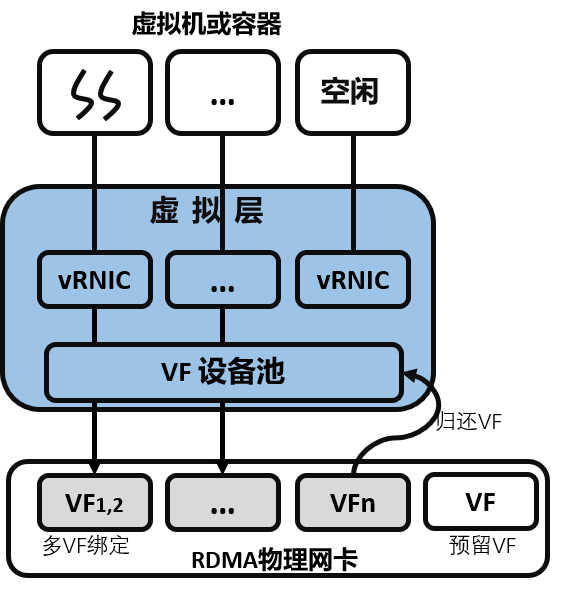
\includegraphics[width=0.9\linewidth]{images/vf-mapping}
	\caption{Management of vRNIC Mapping}
	\label{fig:vf-mapping}
\end{figure}

As Figure~\ref{fig:vf-mapping} shows: First, the virtual layer constructs a dynamic VF pool. The initial number of VFs in the pool is usually the number of pre-determined virtual instances. If lack of free VFs in the pool, the device pool can dynamically expand the number of VFs. Second, the virtual layer supports dynamic mapping between vRNIC and VF. When all virtual RDMA resources have been destroyed, the virtual layer marks the VF as idle and puts it back into the pool. So that the virtual layer can support the number of vRNICs that exceed the VF limit. Finally, the virtual layer supports various mapping relationships between vRNICs and VFs. For example, load balancing can be meted by map a vRNIC with multiple VFs. VF resources are saved by mapping multiple vRNICs of the same virtual instance to the single VF. 


\subsection{Virtual RDMA Management}
To maintain portability and realize RDMA network management, RDMA connections between vRNICs cannot be established by the physical address of VFs. But this problem has a solution that uniRDMA virtual layer acts as a software RDMA switch or router for virtual RDMA network configuration and routing management, etc.

RNICs are usually managed by the subnet manager in the cluster. For the same purpose, a control center is set up in uniRDMA to assign virtual RDMA addresses vGIDs to each vRNIC and configure routing rules between vRNICs. As shown in Figure~\ref{fig:route-config} , the vRNICs are divided into two groups: group 1 and group 2; vRNICs in the same group are allowed to establish RDMA connections, and cross-group RDMA connections cannot succeed due to the isolated routing rules between group 1 and group 2.

\begin{figure}[!ht]
	\centering
	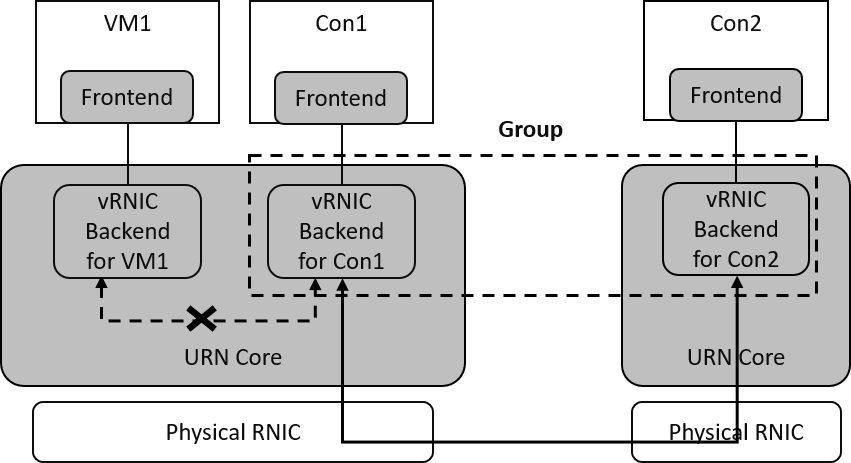
\includegraphics[width=1.0\linewidth]{images/route-config}
	\caption{Virtual RDMA Network Routing}
	\label{fig:route-config}
\end{figure}

Consistent with native RDMA, vRNICs in each virtual layer need to exchange each other's virtual RDMA addresses, virtual QP queue information, registered memory keys and other information to establish virtual RDMA connections. However, the vRNIC RDMA address is virtual, and does not recognized in RNIC. Therefore, the mapping relations between the virtual addresses of vRNICs and the physical addresses of VF needs to be exchanged between virtual layers. When establishing the virtual RDMA connection, the virtual RDMA address is converted to the physical address of the mapped VFs. Note that RDMA resources information, such as virtual QP number and memory keys, have been mapped to the VF interface by the map unit in vRNIC, they can all be recognized VF and directly used to create RDMA connection.

\subsection{Discussion}
Note that all vRNICs (including vRNICs' RDMA resources) are manipulated in the virtual layer. Thus, in virtual layer, there are avaliable for more managements. And we introduce some ongoing features for clouds:

Control police for clouds: To manage the resources precisely, there are lots of important polices in clouds, e.g. QoS, metering and so on. In uniRDMA, we can still meet these control features in virtual layer for these resons:  First,  the virtual layer can monitoring the QPs or CQs for RDMA traffic information, such as,  size and status of one RDMA work request, because all RDMA resources (including QPs and CQs) are mapped at host's virtual layer; Second, the virtual layer can  control the virtual RDMA traffic by controling the RDMA resources,  with the help of host RDMA libraries. For an example,  we can destroy the QP in the virtual layer when a RDMA connections' traffic is excessive.  These will cause more CPU overhead in the host virtual layer, but would not impact the performance of RDMA applications in clouds.
	
Virtual Instances Migration: Migration is important  for both containers and VMs in clouds with many benifits, e.g. resource utilization and fail-over. With the virtual RDMA network , uniRDMA can support offline migration without reconfiguring the physical RDMA network for applications. In specific,after rebooting the migrated virtual instance, the application can rebuild the RDMA connection  only by modifing the address mapping in software virtual layer. Currently, for live migrations, it is still hard because memory regions in RDMA application may be uncertain under bypassing or one-side communication. Thus, uniRDMA does not support live migrations for both VMs and containers.
	
Other network extensions: RDMA can also be exploited to optimize the performance of other network applications,  such as TCP/IP.  Existing works include vSocket ~\cite{wang2019vsocket}, SockDirect~\cite{li2019socksdirect} so on. In uniRDMA, we can extend the simiar design for socket applications in containers and VMs: unified vNICs and the driver of vNICs in containers or VMs.  The difference in the virtual layer is mainly how to emulate the vNICs based on host RDMA's libraries. 
	
